\documentclass{article}
\usepackage[utf8]{inputenc}
\usepackage[english]{babel}
\usepackage{amsmath}
\usepackage{amssymb}
\usepackage{setspace}
\usepackage{natbib} 
\usepackage{graphicx}
\usepackage{subfig}
\usepackage{comment}
\usepackage[backgroundcolor=pink,linecolor=red]{todonotes}
 \usepackage{fullpage}
\usepackage[hidelinks]{hyperref}
\usepackage{xcolor}


%\singlespacing
\onehalfspacing
%\doublespacing

\newcommand{\plr}[1]{\todo[linecolor=blue,backgroundcolor=blue!25,bordercolor=blue]{#1}}
\newcommand{\jgg}[1]{\todo[linecolor=green,backgroundcolor=green!25,bordercolor=black]{#1}}
\newcommand{\bill}[1]{\todo[linecolor=green,backgroundcolor=yellow!25,bordercolor=black]{#1}}

\begin{document}

\title{The sweet spot for local polygenic adaptation: a case study motivated by stickleback}
\author{Jared Galloway, William A. Cresko, and Peter Ralph}
\maketitle

\textbf{Other title ideas?} (Bad ideas allowed.)

How do stickleback share adaptations between lakes? A simulation study.

A simulation study of gene flow and local polygenic adaptation

A simulation study of gene flow and local polygenic adaptation in stickleback fish

\textbf{Jargon}

effect loci? regions underlying trait value?

names of four allele origin categories

\section*{Abstract}

Threespine stickleback fish provide one of the most striking examples of local adaptation. This hemisphere-wide metapopulation includes both marine populations and a large number of smaller freshwater populations
that have apparently repeatedly adapted to freshwater conditions
often using the same genetic basis.
In this paper, we use simulations motivated by stickleback populations
to examine what amounts of gene flow favor stable metapopulation polymorphism
with allele sharing,
and to further dissect the underlying dynamics.
We find that rapid, repeated adaptation 
using alleles maintained at low frequency by migration-selection balance
(the ``transporter hypothesis'')
occurs over a realistic range of intermediate rates of gene flow,
between slow, independent adaptation with low gene flow
and large migration load at high gene flow.
Rapid adaptation occurs when the freshwater haplotype has been maintained,
through historical introgression, in marine environments without tight linkage to 
marine adapted alleles.
We find $F_{ST}$ scans for adaptive alleles are more likely to succeed with higher rates of gene flow.
The results support existing theory of local adaptation,
and provide a more concrete look at a particular, empirically motivated example.

\section*{Introduction}

% Jared's general notes for formatting
%
% - ``citep'' for ``cite in parentheses''. (and, citations come before the punctuation)
% - in latex, use ` `words' ' to get the open- and closed-double quotes (not the double-quote character)
% - "citet" for "cite, as part of the text"

\emph{intro outline:}
Start off with stickleback: repeated, rapid, parallel adaptation with obvious phenotypes.
But, most species don't seem to have such obviously structured polymorphism: 
what's special about stickleback?
The transporter hypothesis is a mechanism; what's required to make it work?
Other species adapt rapidly in similar ways:
e.g., Darwin's finches and island mice;
do these differ through not having such a big, connected reservoir of genetic variation?
or by not having such a large total population size of the ``other'' habitat?
Or, is this situation more common than we know, with less obvious phenotypes?
Also, can we actually tell what's happening from genetic data?

Recently, multiple instances of similar (parallel) underlying genetic basis of rapid local adaptation has brought about 
questions surrounding the origins and maintenance of genetic polymorphism.
A empirical model is the Alaskan populations of freshwater and marine Ninespine Stickleback fish.
In 1964, The Great Alaskan Earthquake caused an uplift of Middleton island and in turn,
introduced a group of freshwater ponds around the perimeter of the island. 
Quickly inhabited by the surrounding marine population of Stickleback,
\citet{lescak2015evolution} observed significant phenotypic changes in less than 50 years that appear to be 
parallel to freshwater stickleback that have been separated for over $13,000$ years.
In freshwater stickleback, the number of lateral plates are reduced
and the opercle shapes shows the same expansion of the dorsal region and reduction of the ventral region.
These results leave us with questions surrounding the nature of rapid adaptation.
Does convergent evolution breed it's own solution (haplotype) for every new selective pressure, 
or can these solutions can be efficiently shared across multiple sub - populations facing similar selective pressures. 

The leading hypothesis for stickleback is that rather than acting on new mutations, 
adaptation to freshwater environments is sped up through selection on standing genetic variation (SGV) found in marine populations. 
\jgg{Bill: maybe you could make this section a little more specific}
One clear example of this is the gene \textit{eda} 
which has been shown to regulate the number of lateral plates. 
While this gene arose millions of years ago, it is found in freshwater ponds which have formed much more recently.
Novel evidence from natural populations has provided evidence that most regions of the genome that distinguish marine-freshwater genetic differences share this pattern \citep{nelson2017ancient}.
\citet{schluter2009genetics} 
suggested the ``transporter''-hypothesis.  
This outlined the flow of freshwater alleles into marine populations through offspring of hybridization events.
It suggests freshwater haplotypes are distributed though marine individuals and are continually selected upon in introduced freshwater populations.
The continued selection on freshwater favored alleles and introgression between the two sub-species,
allows the marine to maintain the freshwater haplotype dispersed in low frequency among its' individuals. 
Once a new freshwater environment is introduced and inhabited by marine individuals who carry freshwater adapted alleles, selection reconstructs the freshwater haplotype \citep{schluter2009genetics}.
An alternative to this hypothesis is that individuals from other freshwater environments migrate directly to the new environments, 
and their haplotype is passed down directly. 
This hypothesis has been shown to be unlikely due to finding a high frequency of freshwater alleles in the ocean,
and almost no freshwater individuals.

\plr{Bring up the possibility of more than one freshwater haplotype here.}
\jgg{Re: should I? Doesn't Thom's work and parallel above suggest they have the same alleles?}

If selection on standing genetic variants is key in rapid adaptation, 
many questions are exposed concerning the surrounding population genetics parameters and underlying genomic architecture.
%How rapidly can selection act on standing genetic variants at a given value of migration, $M$?
What scale of historical introgression between populations with selective pressures $X$ and $Y$, allows for rapid and parallel local adaptation
of a population derived from $X$ to an introduced environment with selective pressure $Y$?
What is the origin of pre-existing adaptive variants?
How are the variants structured, historically and across the genome underlying the trait?
%How does population genetics data influenced by historical introgression and selection on standing genetic variants?
%How many alleles underly a certain trait and how many are swept away by drift? 
Furthermore, how can we infer causal loci for regions of the genome that must be driving the rapid adaptation, from real data.
Many biologists today make use of genome wide association studies (GWAS) and 
$F_{st}$ across the genome to estimate regions responsible for certain traits. 
Unfortunately, the data can be heavily influenced by the level of introgression and population structure of the samples. 
This being the case, what are the biases we can expect to see in real data for certain levels of introgression. 

There are many different parameters that carry a large impact on the questions above.
\citet{ralph2015convergent} 
explored the dichotomy of selection on new alleles and those brought in by migrants from a similar selective pressure.
Answering the fundamental questions surrounding spatial resolution of convergent evolution. 
%This lead to an understanding of the process by which alleles move from an existing 'patch' to an introduced 'patch' with the 
%same selective pressure. 
\jgg{It seems like this could be a good parallel to what we're doing here, or maybe for discussion?}

In this paper, we explore time to local adaptation as a function of migration rate through an environment (marine) with opposing selective pressure. 
Next, we compare to real data and explore how $F_{st}$ data can be impacted by introgression.
%Explain what we do and what we find that is important

%We use forward moving simulations to model marine and freshwater populations of stickleback.
%We then observe the effect (focusing on migration and recombination, for now) 
%of different parameters on local adaptation of introduced freshwater environments. 


%%%%%%%%%%%%%%%%
\section*{Methods}

We explored these questions
using forwards-time simulations with explicit genomic representation of a quantitative trait
in SLiM \citep{haller2017slim}.
The details (described below) are motivated by previous population genomic studies of threespine stickleback,
but remain simplistic in some aspects due to computational constraints.
\jgg{should we brag about treeSeq here a little?}
Possibly the most important caveat is that simulated population sizes are much smaller
than the census size of the Threespine Stickleback population;
we will consider the likely effects of this in the Discussion.
\plr{TODO}

\paragraph{Habitat and geography}
Our model has two habitat types, which are considered separate populations
with a fixed total size of 5,000 diploid individuals each. The marine population is treated as a single large deme, but the freshwater population is subdivided into local subpopulations or demes.
The scheme, depicted in Figure \ref{fig:Geo},
roughly models a set of freshwater habitats
along a stretch of coastline.
The ``marine'' habitat  is a continuous, one-dimensional range of 25 units of length,
and the ``freshwater'' habitat is divided into ten subpopulations
(which we call ``lakes''), each connected to the marine habitat
at positions $i - 1/2$ for $1 \le i \le 25$.

Fitness in each habitat is determined by a single continuous trait with an inherent tradeoff such that alternative values of the trait have high or low fitness in the two different habitats. This situation roughly models the cumulative effect of the various phenotypes
such as armor morphology, body size, craniofacial variation and opercle shape (among others)
on which divergent selection acts in the two environments.
The optimal trait value in the marine habitat is $+10$,
and in the freshwater habitat is $-10$. Fitness of a fish with trait value $x$ in a habitat with optimal value $x_\text{opt}$ is
Gaussian with standard deviation, i.e.,
\begin{align*}
    f(x; x_0)
    &=
    \exp\left\{
        \frac{1}{2}
            \left(
            \frac{x-x_\text{opt}}{15}
            \right)^2
        \right\} .
\end{align*}

\begin{figure}
	\begin{center}
  		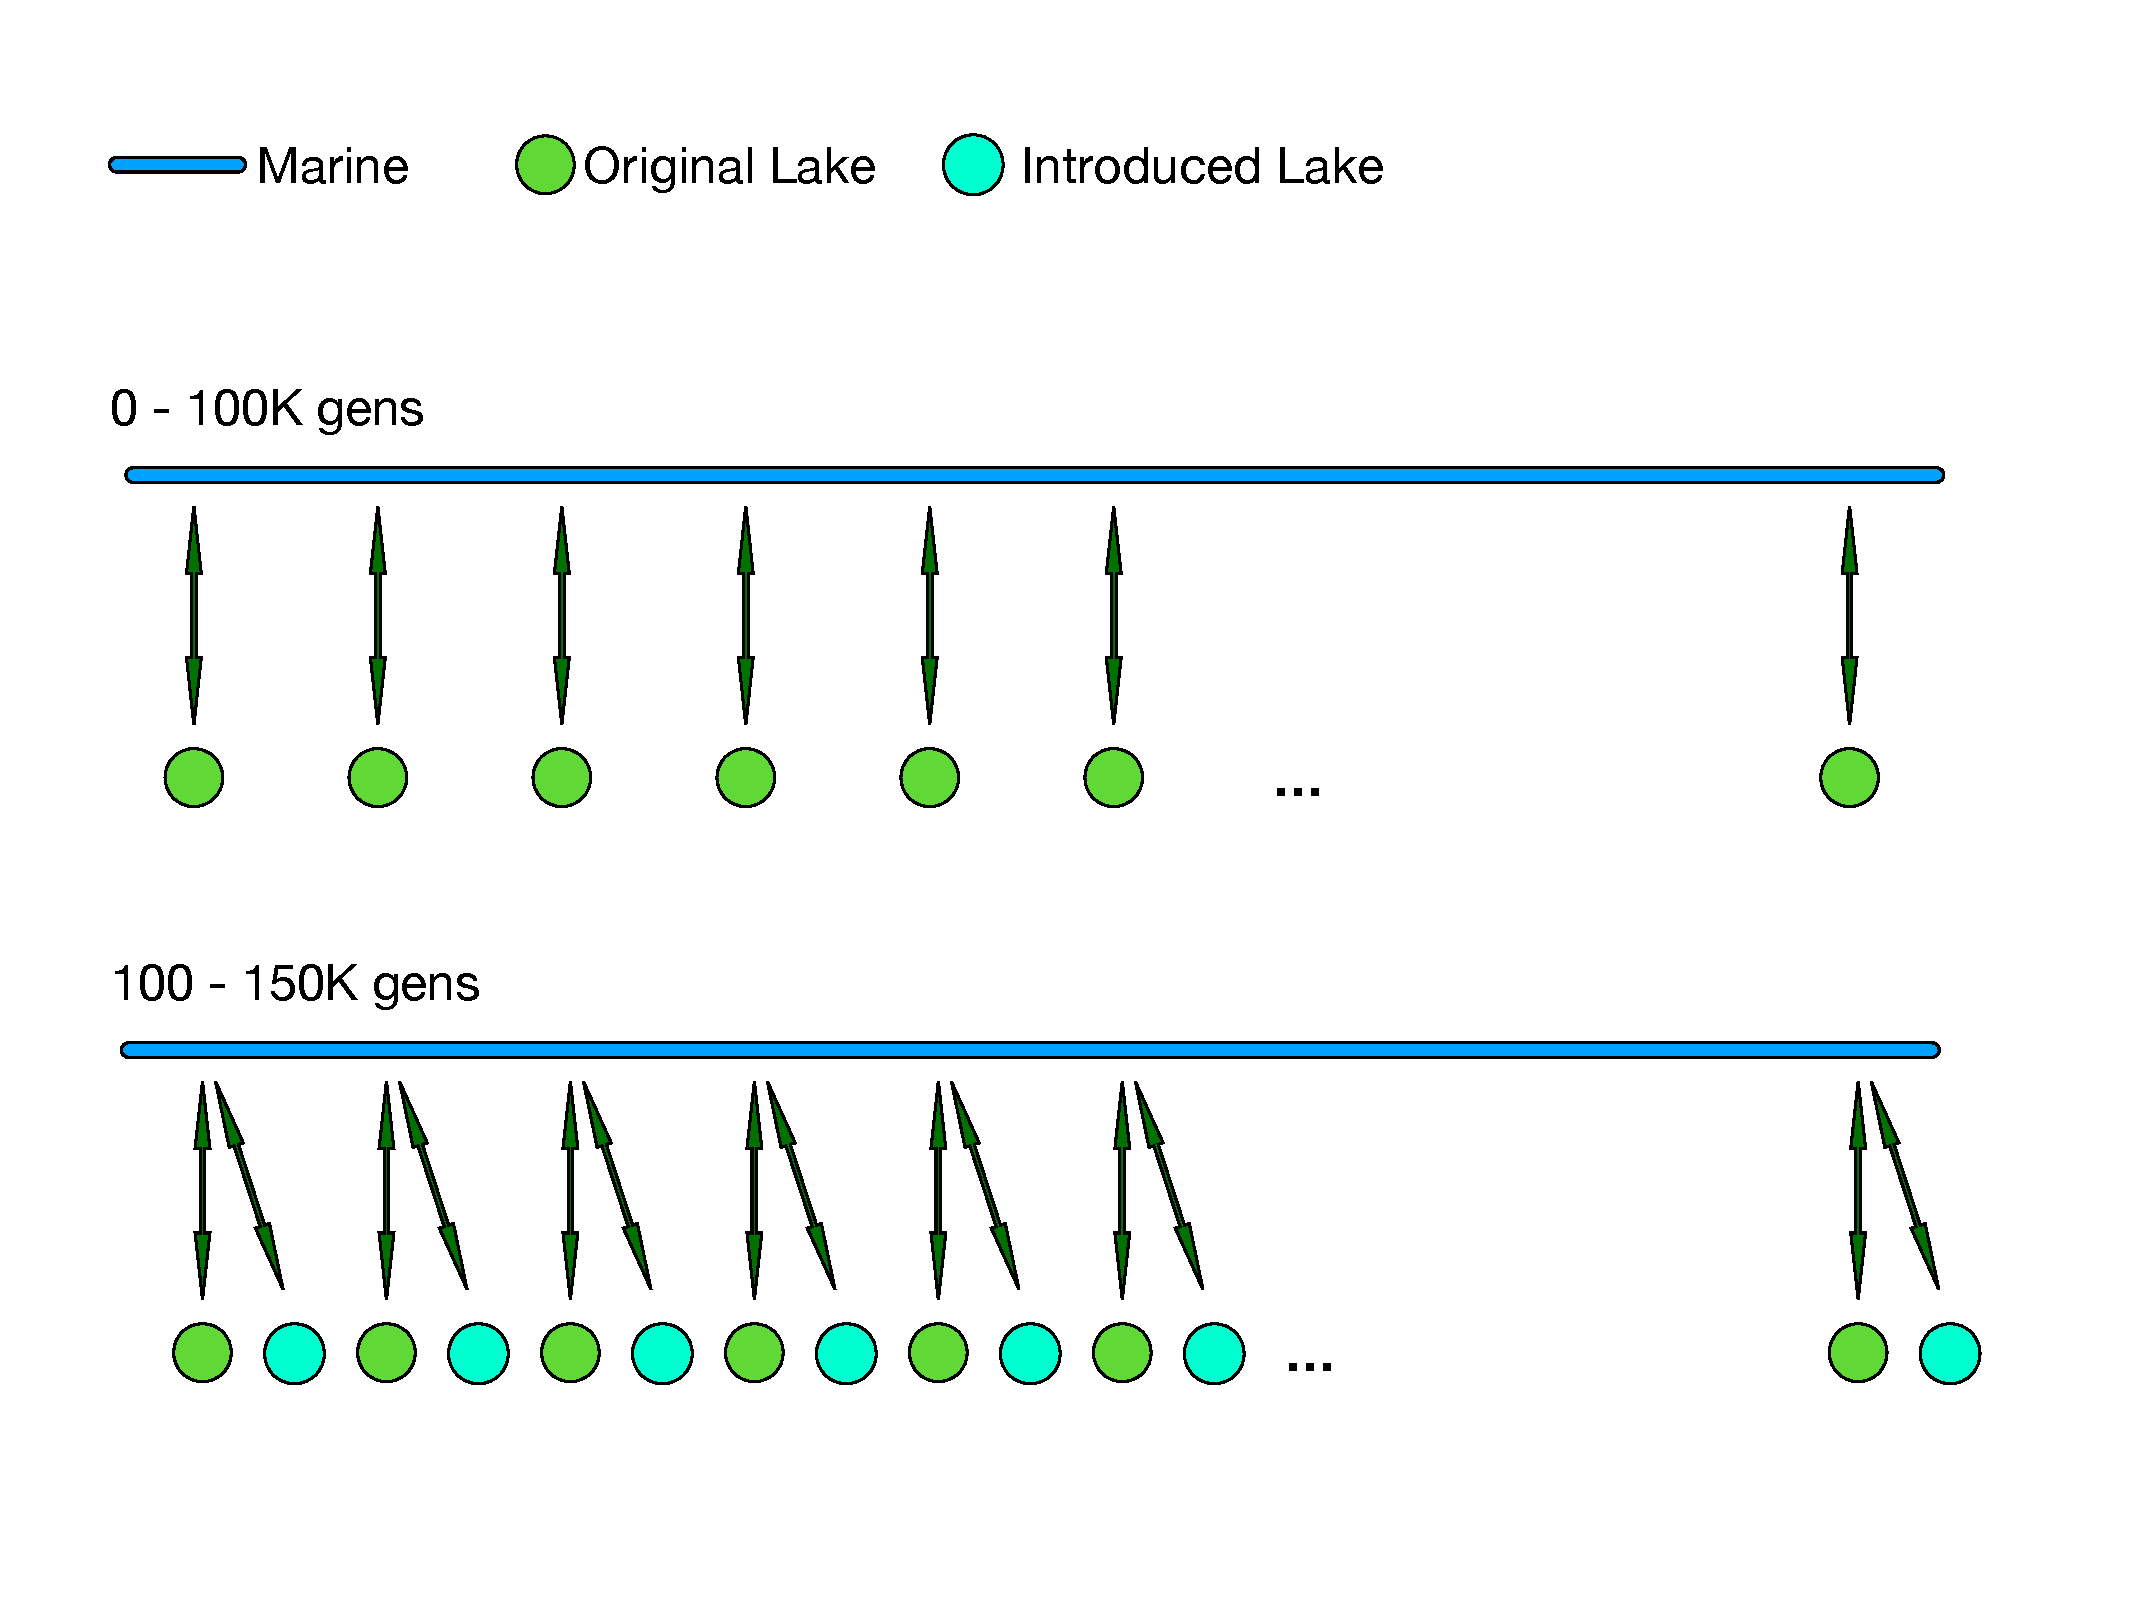
\includegraphics[width=0.6\linewidth]{GeographyFigure.pdf}
  		\caption{
			A representation of the geographic and evolutionary history of all populations throughout the simulation. 
		The marine is a one-dimensional, continuous population with spatial positions ranging from [0.0 - 25.0]. 
		Each freshwater lake$_{i}$ for both the introduced and freshwater populations
		is a discrete population connected by migration only through the marine, at position $i - 0.5$. 
		Each of the introduced lakes have the same spatial dynamic and selective pressure as the pre-existing lakes, but arise at 100K generations into the simulation.
		The marine has $5000$ diploid individuals while each of the lakes fluctuate  $200$ diploid individuals. 
		the introduced population is initialized as a copy of all marine individuals to model marine 
		individuals inhabiting a newly created freshwater environment such as the ponds around Middleton Island.
		We then observe the selection process of marine individuals and following generations 
		with the new selective pressure across a range of parameter values. 
			}
  		\label{fig:Geo}
	\end{center}
\end{figure}

\paragraph{Potential genomic architecture}\bill{Initial genomic architecture? The header is a little confusing to me}
Each individual carries two copies of a linear chromosome of $10^8$ loci representing a realistic size genome.
New mutations occur with probability $10^{-10}$ per locus per generation in regions affecting phenotype and $10^{-8}$ in neutral regions.
Ten ``effect regions'' of $100 Kb$  loci each are spread evenly along the chromosome; 
mutations in these regions have the potential to affect trait value of the individual which posses them.
Each mutation in these regions is either additive, completely recessive,
or completely dominant (with equal probability).
Effect sizes are chosen randomly from an exponential distribution with mean $1/2$,
either positive or negative with equal probability.
Between the effect regions is $9.9 Mb$ of neutral loci.
Individual trait values are determined additively from the diploid genotypes.
Concretely, an individual that is heterozygous and homozygous for mutations
at loci $H$ and $D$ respectively has trait value
$x = \sum_{\ell \in H} h_\ell s_\ell + \sum_{\ell \in D} s_\ell$,
where $s_\ell$ is the effect size of the mutation at locus $\ell$.
Subsequent mutations at the same locus replace the previous allele.

\paragraph{Life cycle}
Each generation, the two parents of each new offspring are chosen 
proportional to their fitness (all individuals are hermaphroditic),
and the contributing genomes are produced by Poisson recombination
with an average of one crossover per chromosome per generation
($10^{-8}$ per locus per generation).
The model is Wright-Fisher, so that each generation, in each habitat,
5000 new individuals are produced,
and so to keep population sizes roughly constant within each lake,
at the start of each generation we rescale fitness values in the freshwater habitat
so that the sum of the fitness values within each lake are equal.

Migration occurs both locally along the coastline in the marine habitat
and between the marine habitat and the lakes,
and can be thought of as occurring at the juvenile stage.
The between-habitat migration rate is denoted $m$,
and will be called simply the ``gene flow''.
$\approx m$ individuals \emph{per} lake \emph{per} generation, have parents from the opposing selective pressure.
A first parent is chosen proportional to fitness,
and a mate is chosen from the same lake as the first, also proportional to fitness.
The resulting offspring is given a spatial location in the marine habitat
at the location of the parent's lake.
Parents for a new marine individual who is not a migrant are chosen similarly (with probability $1-m$):
first, a single parent is chosen proportionally to fitness in the marine habitat,
and then a mate is chosen, 
also proportionally to fitness but reweighed by a Gaussian function 
of the distance separating the two, with standard deviation $1/2$. 
More specifically, if the first parent is marine individual $i$,
then marine individual $j$ is chosen as the mate
with probability proportional to $f(x_i) \exp(-2d_{ij}^2)$,
where $d_{ij}$ is the distance between the two locations.
Finally, each new marine offspring is given a position 
displaced from the first parent's position by a random Gaussian distance
with mean 0 and standard deviation 0.02, and reflected to stay within the population.
New offspring in the freshwater habitat are chosen in the same way,
except the probability that the parents are marine individuals is $m$;
any new freshwater offspring produced by marine individuals
are assigned to the lake nearest to the position of the first marine parent.

\paragraph{New lakes}
To study adaptation in newly appearing freshwater habitats,
we introduce a new set of lakes midway through the simulation.
As with the old lakes, these are a set of discrete demes connected by migration \emph{only} to the marine.
The initial generation of individuals in these new lakes were created as a copy of the marine individuals 
at the generation of introduction.
The new lake's geography acts like an independent copy of the original set of lakes -- in particular,
the two sets of lakes each have 5,000 individuals at all times.
%(Gene flow constricted to within the lakes and through migration to the marine environment).
Since this doubles the number of lake-to-marine immigrants,
after this happens the probability that a new marine individual has parents from old lakes or the new lakes
is $2m$ instead of $m$.

\paragraph{TreeSeq}
This case study involves analyzing large simulations which model populations under the influence of selection. 
To fully understand the origins of freshwater alleles, calculate statistics, and avoid the computationally expensive task of 
simulating neutral mutations, we have used SLiM's \emph{treeSeq} feature to track the genealogical history of all samples throughout the simulation. 
This feature outputs a compact representation the genomic outcome of every meiosis relevant to tracked samples (Often thought of as the ARG).

Using the output tree sequence, 
we were able to classify each freshwater allele in each genome of the new lakes population, at time of adaptation,
as deriving from one of four origins:
(1) Migrants, brought in from a migrant after the introduction of the new lakes 
(2) Pre-existing, passed down from an individual in the original generation of the new lakes, 
however, not defined to be an adaptive variant in the original lakes
(3) Captured, Pre-existing, passed down from an individual in the original generation of the new lakes, 
and defined to be adaptive in the original lakes
(4) De novo, mutated and propagated from an individual existing in the introduced lakes population, after introduction. 
\jgg{We should discuss further what these categories aught to be named}

\begin{comment}
We also used the tree sequence to count the "fitness" of individuals in the initial generation of the new lakes. 
The "fitness" of an individual in this case, is defined to be the total number off eventual offspring, in the generation at the time of adaptation, 
which have inherited a adaptive variant from that individual. 
To calculate this, we only considered gene trees which overlapped an adaptive variant site (defined at time of adaptation).
We then counted the total number of offspring which had inherited from any adaptive variant site, 
for each individual in the initial generation. 
\end{comment}

We were also able to use the tree sequence to get information about the individual ``effect regions" 
in all initial genomes of the new lakes at time of introduction.
From this we determined the ability for the new lakes to select upon the standing variation in the marine.
Given the probability that effect region fixes at a given trait value, $2 * x / 45$, where $x$ is the effect size of a haplotype,
we calculated the expected total effect sizes of the haplotypes that fix.
Concretely, it is the sum across the 10 effect regions of
$$\sum_{i=1}^N \prod_{j < i} (1 - p_j) p_i x_i$$
where $N$ is the number of genomes per lake, $p_i$ is the probability of fixation of the 
$i^{th}$ haplotype, $x_{i}$ is the effect size of the $i^{th}$ haplotype, and the haplotypes are sorted in decreasing order by $x_{i}$.
These numbers were computed assuming additivity of mutations, meaning the numbers produced are a slight overestimate.

\paragraph{Descriptive statistics}\bill{Population genetic analyses? Instead of the more general 'Descriptive statistics'?}
To assess whether new lakes adapt using existing genetic diversity,
we define a \emph{freshwater allele}
to be an effect mutation that has frequency higher than $0.5$ in at least one of the original lakes,
while remaining lower than $0.5$ in the marine. 
This categorization is made for each generation using the allele frequencies from that generation,
and so changes with time.
Alleles common in the newly introduced lakes do not count
if they are not also common in the original lakes.
They are defined this way because the transportation hypothesis 
does not specify where or when an advantageous mutation arises,
but simply suggests that any sufficiently common freshwater adapted allele 
could participate in adaptation in new habitat \citep{schluter2009genetics}.

\emph{Time to adaptation} of the introduced population, denoted $T_\text{adapt}$, 
is defined to be the generation at which 
the difference between the average trait value in the original and the introduced freshwater populations 
is less than 0.5. 

We describe overall genetic differentiation between the habitats using $F_{ST}$,
calculated on a per-locus basis.
Concretely, if $p_f$ and $p_m$ are the frequencies of a given mutant allele
in the freshwater and marine habitats, respectively,
and $\bar p = (p_f + p_m)/2$,
then we compute $F_{ST}$ for that mutation as $1 - p_f p_m / (\bar p (1-\bar p))$.

\section*{Results}

We varied the migration rate, $m$ across separate simulations
from $5 \times 10^{-5}$ to $5 \times 10^{-1}$ by one order of magnitude steps.
For clarity given our populations sizes of 5,000 diploid individuals, 200 in each lakes,
we will refer to these rates of gene flow as running simulations ranging from {0.01 - 100.0}
migrants \emph{per} lake \emph{per} generation.
The differing parameter values had a strong effect on many aspects of adaptation;
including how fast adaptation occurred in each lake,
how many alleles were shared between lakes,
and the population genetic signals left behind.
We find a threshold of gene flow which allows 
the freshwater haplotype to be maintained in the marine without creating linkage to marine alleles. 
below this threshold, selection on pre-existing freshwater alleles to be much less efficient 
due to background selection. \jgg{did I get this right?}

Interestingly, all rates of $m$ aside from the two highest had little affect on population's ability to locally adapt.
All rates of gene flow aside from the lowest, helped both the old lake's and the new lake's freshwater populations share pre-existing freshwater adapted alleles.
The sharing of alleles at $m = 1.0$ resulted in rapid adaptation ($\approx 32$ generations) of the introduced population to adapt to the freshwater environment.
At the lowest migration rate, lakes adapted nearly independently,
while at the highest migration rate, the habitats act like a single metapopulation
with substantial migration load.
We will now dissect what happens between these extremes.

\subsection*{Local Adaptation: differentiation with gene flow}

\begin{figure}
	\begin{center}
        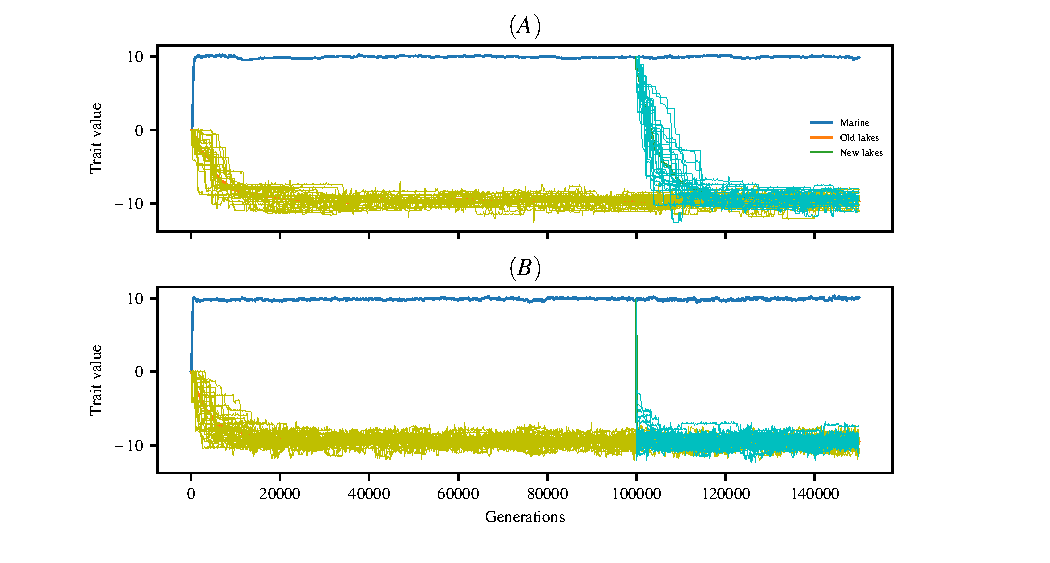
\includegraphics{Final_Plots/Pheno_Time.pdf}
  		\caption{ 
        		Mean individual trait values in the marine habitat (blue line),
        		the original lakes (light green lines; average in dark green),
        		and the introduced lakes (yellow lines; average in orange)
        		across the course of two simulations, with migration rates of
        		\textbf{(top)} $m=5 \times 10^{-5}$ and
        		\textbf{(bottom)} $m=5 \times 10^{-4}$ per generation individual
        		(i.e., 0.01 and 0.1 migrants per lake per generation, respectively).
        		Optimal trait values in the two habitats are at $\pm 10$.
		}
  		\label{fig:phenotype_ts2}
	\end{center}
\end{figure}

Local adaptation occurred in all simulations:
as shown in Figure \ref{fig:phenotype_ts2},
freshwater and marine populations diverged
until the trait means were close to the optimal values in each habitat. 
The establishment of new alleles in the lakes is visible in Figure \ref{fig:phenotype_ts2}
as jumps in the mean trait value;
in the two simulations these occur on a time scale of 100 (lower migration) to 1000 (higher migration) generations,
\jgg{I'm not sure what this means? how do we know how long the jumps take?}
and move the trait by an amount of order 1.
Trait variation within each population was small compared to the difference between populations,
with interquartile ranges of around XXX.\plr{TODO}
Across all parameter values, differences at around 16 commonly polymorphic sites 
(eight the shift the trait in each direction)
were responsible for most of the adaptive differences between freshwater and marine habitats.

As expected, increasing migration rate decreased differentiation between habitats.
As seen in Figure \ref{fig:Fst},
$F_{ST}$ between marine and freshwater habitats at neutral sites 
steadily declines as migration increases.
Local adaptation was still able to occur despite overall homogenization:
if computed using only sites with alleles affecting the trait (``effect mutations''),
$F_{ST}$ between habitats was relatively constant across migration values.

\begin{figure}
	\begin{center}
  		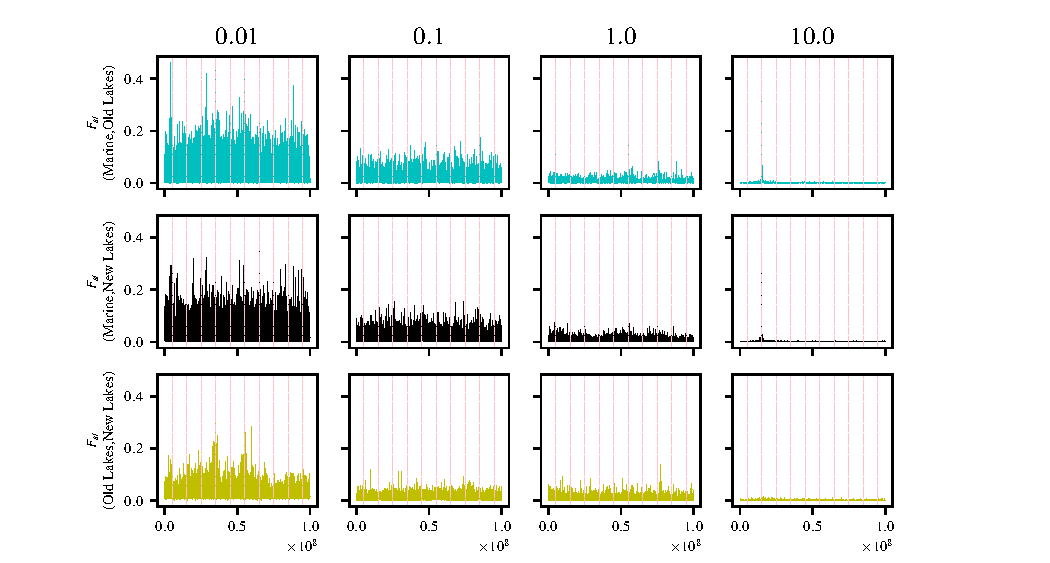
\includegraphics{Final_Plots/Fst_Genome.pdf}
  		\caption{
		$F_{st}$ as a function of genomic location between all combinations of the three subpopulations; 
		the old lakes, the new lakes, and the marine.
		$F_{st}$ was calculated based upon allele frequencies in genomic windows of 500 mb. 
		The four columns of subplots are separate simulations with increasing $m$. 
		The three rows are the combinations of the three separate populations.
		Ten vertical dotted pink lines in each subplot represent regions which have the potential to affect phenotype
		 }
  		\label{fig:Fst}
	\end{center}
\end{figure}

\paragraph*{Speed of adaptation}
Increasing migration rate strongly decreased the time until freshwater habitats could adapt,
both in the old and new sets of lakes.
The different rates of introduction of effect alleles is clearly seen in the traces
of trait values against time (e.g., Figure \ref{fig:phenotype_ts2}).
As shown in Figure \ref{fig:TimeToAdaptation}, at the lowest migration rate 
it took over $18,000$ generations for the mean trait value across introduced lakes to 
get to within 0.5 of the original lakes value.
At $m = 1.0$, we saw the introduced population adapt in just $32$ generations. 
This rate of adaptation follows what we've observed in natural populations of threespine stickleback.
At the highest migration rate, $m = 100$, all individuals were unable to locally adapt.

\begin{figure}
	\begin{center}
  		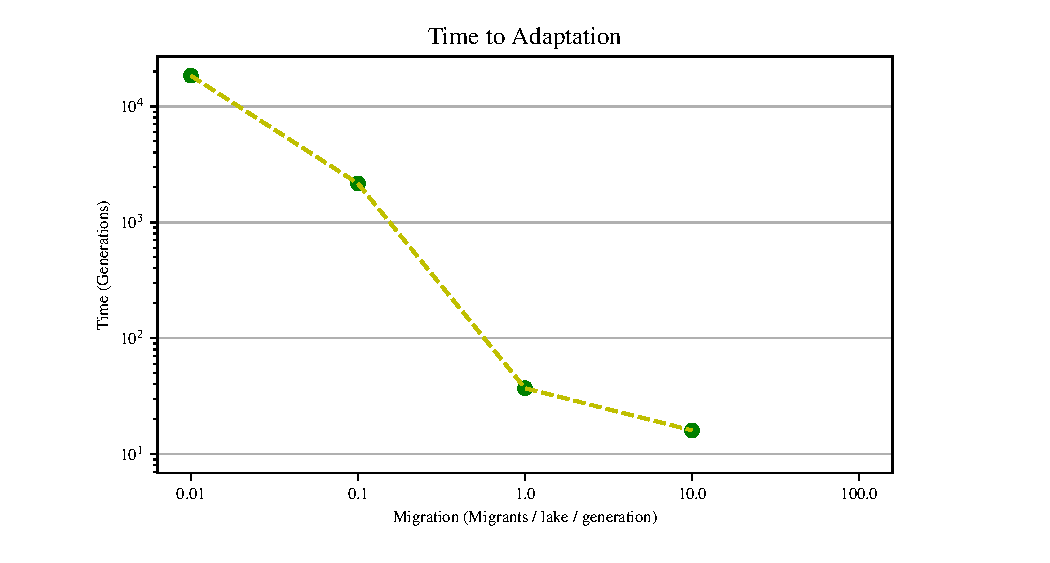
\includegraphics{Final_Plots/Time_Adapt.pdf}
  		\caption{
		Time to adaptation as a function of migration rate ($M$) parameter value. This is where we measure how many generation
		it takes for the introduced population's mean phenotype to come within 0.5 of the original lakes average phenotype. 
		Each point represents a simulation run at some value of $M$. 
		The yellow dashed line is the average of all points at each respective parameter value}
  		\label{fig:TimeToAdaptation}
	\end{center}
\end{figure}

\subsection*{Sharing of freshwater alleles}

We find that this dramatic increase in speed of local adaptation occurs because
higher gene between populations allow sharing of freshwater alleles more effectively when compared to de novo mutation.
At low migration rates, adaptation occurs independently in each lake.
In Figure \ref{fig:Origin}, at $0.01$, we can see that the large majority of adaptive alleles derived from de novo mutation in the 
population rather than selection on standing variants in the ocean. 
As The migration increases, we see a larger ratio of the origins of adaptive alleles 
derive from pre-existing variation in the marine population at the time of introduction.
In other words, 
greater mixing at higher migration rates allows lakes to share alleles
instead of developing their own genetic basis of adaptation.
To further investigate sharing of locally adaptive alleles and the transporter hypothesis,
we investigate the ``freshwater alleles'', defined for a particular generation
to be effect mutations above 50\% in at least one original lake and below 50\% in the marine habitat in that generation.

As the number of common, locally adaptive alleles decreases, as seen in Figure \ref{fig:MPFAI}C,
the genetic basis of adaptation is more commonly shared.
Figure \ref{fig:MPFAI}B shows
the percentage of currently-defined, freshwater-adapted alleles 
that each genome in each of the populations carries,
averaged across time and individuals.
If all individuals across lakes carried the same set of alleles determining their trait value,
this would be 100\%.
This value is nearly reached at the fourth migration rate;
but it is lower due to migration load.
At the lowest migration rate, 
each genome in the original lakes have almost exactly $1/25^{th} = 0.04\%$   
of the total freshwater adapted alleles --
since there are 25 lakes, this implies that each lake has adapted with a unique set of alleles.
Since these are \emph{pre-existing} alleles, the value is zero for introduced lakes.
Figure \ref{fig:MPFAI}A shows us that by $0.1$ migrants per lake per generation,
the average individual across the new lakes has nearly the same amount of 
``pre-existing freshwater adapted alleles" as individuals across the old lakes.
Interestingly, the genetic basis of the freshwater phenotype 
seems to simplify with greater $m$. 
This would seem to suggest higher rates of migration allowed 
adaptive alleles of higher effect to travel more efficiently through the populations
\jgg{is this right?}

\begin{figure}
	\begin{center}
  		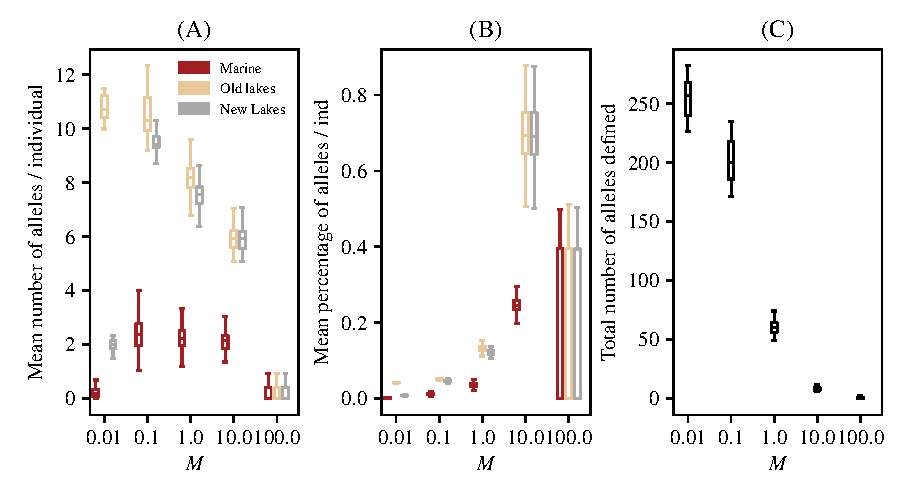
\includegraphics{Final_Plots/Freshwater_Alleles.pdf}
  		\caption{
		Distribution of freshwater alleles among the three populations. 
		A freshwater adapted variant is defined as, at any generation throughout the simulation,
		a variant affecting phenotype that is greater than 0.5 frequency in any of the old lakes, 
		and less than 0.5 frequency in the marine population. 
		Subplot $A$ is the distribution throughout the simulation, of the mean number of
		freshwater adapted variants per individual, in each population.
		Subplot $B$ is the distribution throughout the simulation, of the mean \emph{percentage} of
		freshwater adapted variants per individual, in each population. 
		Subplot $C$ is the distribution throughout the simulation, of the total number of
		freshwater adapted alleles defined at any one generation.
		In other words, $B  =  A  /  C$.
		}
		\label{fig:MPFAI}
	\end{center}
\end{figure}

\subsection*{Migration load and genetic variation}

At first, increased migration allows sharing of adaptive alleles between lakes,
but at $m = 5 \times 10^{-2}$
the constant influx of alleles between the habitats creates noticeable migration load.
This rate, $m=.05$, only replaces 5\% of each population each generation
with migrants from the other habitat, but this is sufficient to shift the mean trait values
to nearly half their optimal values, as seen in Figure \ref{fig:MeanPhenotype}.
Significant gene flow constricts local adaptation
as a consequence of a large number of offspring through hybridization events between subpopulations.
at $m=0.5$, all populations experience panmixia 

\begin{figure}
	\begin{center}
  		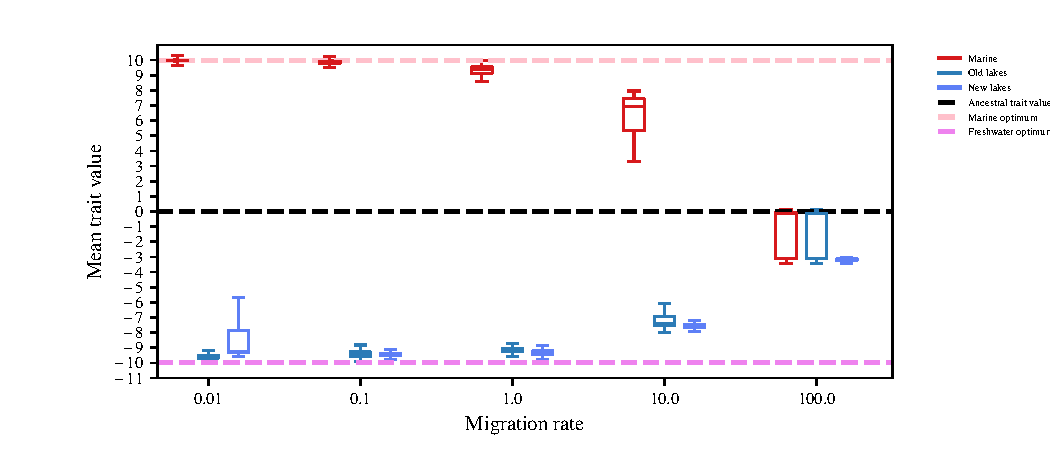
\includegraphics{Final_Plots/Pheno_Dist.pdf}
  		\caption{Distribution of mean trait value throughout simulation runs at separate migration rate $(m)$ parameter values, for each population.
		The dashed pink line (Trait value = +10) is the optimum phenotype any individual in the marine environment.
		In contrast the purple line at (Trait value = -10) represents the optimum for any individual in the freshwater environment. 
		All individuals at generation 0 (beginning of the simulation) 
		}
  		\label{fig:MeanPhenotype}
	\end{center}
\end{figure}

\subsection*{Realized genomic architecture}

Higher migration rates showed more distinct $F_{ST}$ peaks
over polymorphic loci underlying trait differences between the habitats.
As migration rate decreased, the ``background'' levels of $F_{ST}$ increased,
swamping out this signal until the regions under selection were indistinguishable. 
This is likely due to two reasons: 
first, stronger genetic drift with less migration leading to higher background $F_{ST}$,
and second, greater sharing of adaptive alleles providing a shared signal across populations.
This suggests that genome scans for local adaptation
based purely on measures of differentiation
will only be successful given enough migration between habitats.
With 10 effect regions across the genome, we can see in \ref{fig:Fst} that only about 1 or 2 of the region contain peaks. 
When looking closely at the peaks we see that each is usually a composition of 7-8 SNPs close in proximity.
Because some of those mutations are selectively neutral (we can see this because the counts of FAA are not as high as the number in the clusters),
this is suggestive of hitchhiking alleles along with the SNPs being brought to high frequency by a selective sweeps.

Given that migration increases the gene flow between subpopulations, how valid are $F_{st}$ peaks at different $M$?
Knowing exactly which mutations effect phenotype in our simulations, 
we can look at the statistical power and false positives given $F_{st}$ per SNP across the genome. 
In Figure \ref{fig:Power_FP} , looking at an $F_{st}$ threshold greater than 1, 
we see the two lowest migration rates $10^{-5}$ and $10^{-4}$ having very little statical power. 
This along with low false positive rate across all $F_{st}$ threshold values is fairly predictable when you consider the high $F_{st}$ values across the genome. 

\subsubsection*{Origin of introduced freshwater adaptive alleles}
Up to this point, we have quantified rapid adaptation and found strong evidence that sharing of alleles is responsible in this system.
Interestingly, in Figure \ref{fig:MPFAI}A at $m = 0.1$, we see sharing of alleles between populations,
yet \emph{Time to adaptation} is still fairly slow ($\approx 2,000$ gens).
This is surprising when considering we see a similar quantity of allele sharing at  $m = 1.0$, 
but much more rapid adaptation ($\approx 30$ gens). 
Initially, this 60X speedup of adaptation seems to be the result of subsequent gene flow of freshwater alleles. 
Perhaps a larger influx of freshwater alleles are needed in addition to standing variation in the initial generation.
To investigate this further we have tracked the origins of all freshwater alleles, in all new lake individuals at the time of adaptation. 
Surprisingly in Figure \ref{fig:Origin}, we find that at both $m = 0.1$ and $m = 1.0$,
the vast majority of adaptive alleles were found to propagate from individuals in the original generation ("Captured" OR "Pre-Existing").

\begin{figure}
	\begin{center}
  		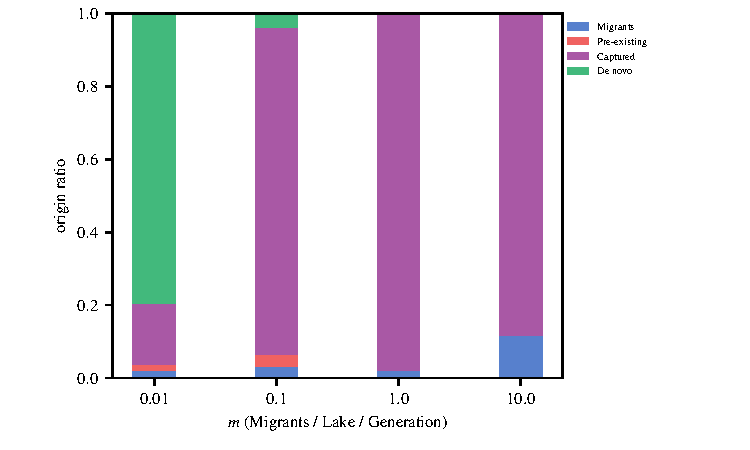
\includegraphics[width=0.7\linewidth]{Final_Plots/Allele_Origin.pdf}
  		\caption{ 
		Origin ratio of adaptive alleles in all genomes at time of local adaptation for different values of $m$
		For all alleles at a frequency $> 0.5$ in any one of the new lakes individuals at time of adaptation, 
		we traced the origin of the segment of DNA back in time to classify them as 
		\textbf{(Blue)} Migrants, brought in from a migrant after the introduction of the new lakes 
		\textbf{(Orange)} Pre-existing, passed down from an individual in the original generation of the new lakes, 
		however, not defined to be an adaptive variant in the original lakes
		\textbf{(Green)} Captured, Pre-existing, passed down from an individual in the original generation of the new lakes, 
		and defined to be adaptive in the original lakes
		\textbf{(Red)} De novo, mutated and propagated from an individual existing in the introduced lakes population, after introduction. 
		}
  		\label{fig:Origin}
	\end{center}
\end{figure}

The alternative explanation, is that at a lower migration rate, a higher saturation of marine adapted alleles are linked to freshwater adapted alleles.
In turn, the equilibrium of freshwater alleles in marine genomes created by migration-selection balance acts as a barrier when rebuilding the freshwater haplotype. 
%With more gene flow between the two selective pressures, the freshwater haplotype remains more "intact" and much more efficient to rebuild in the introduced environment.
To confirm this, we decided to look at the trait values of the ten affect regions in each genome of the initial population.
Given the probability that an ``effect region" fixes at a given trait value, $2 \times x / 45$ where $x$ is the effect size of a haplotype,
we were able to determine expected total effect sizes of the haplotypes that fix (detail about computation in methods).
Below, we see the mean of these expected total effect sizes across all lakes.

\begin{center}
\begin{tabular}{ | c | c  | c  | c | }
 \hline
 $m = 0.01$ & $m = 0.1$ & $m = 1.0$ & $m = 10.0$ \\ 
 $-0.1227$ &  $-4.6976$ & $-12.9298$  & $-12.2710$\\
 \hline
\end{tabular}
\end{center}

Between $m = 0.1$ and $m = 1.0$ we see a large difference in the total effect sizes of the haplotypes that are expected to fix.
Given these numbers were computed assuming additivity (slight overestimate) and individuals are diploid,
at $m = 0.1$ the mean total genotype expected to fix in the populations puts individuals at a trait value of $\approx -8$ 
after selection on alleles haplotypes in the initial population. 
In turn, the population must wait for novel mutation or subsequent migration to provide the alleles for the remaining 2 units before 
attaining a mean average trait value at the optimum (-10).
It follows in Figure \ref{fig:phenotype_ts2}B that the majority time to adaptation is spent within 2 units of mean trait value.
The initial adaptation on selection of standing variation up to that point happens quite rapidly.
This provides evidence that linkage to marine alleles has a major impact in the introduced population's ability 
to select and rebuild a pre-existing haplotype given the standing variation at time of introduction. 

\subsection*{Theoretical expectations}
\plr{does this go first or second?}

Here's some rough calculations to get a sense for what should be going on.
Everything is done in more detail in OTHER PLACES WE SHOULD CITE.
Fisher, Chevin, etc.

Suppose a new allele enters a lake, either by migration or mutation.
If, when it is rare but present in $n$ copies,
it has fitness advantage $s$
-- i.e., the expected number of copies in the next generation is $(1+s)n$ --
then the probability that it escapes demographic stochasticity to become common in the population
is approximately $2s$ \citep{fisher,prob_fixation}.
If the current population all differed from the optimum trait by $z$,
and the allele has effect size $-u$ in heterozygotes,
then the fitness advantage of the allele would be
$s(u) = \exp(-\beta((z - u)^2) / \exp( - \beta z^2)) \approx 2 \beta z u$,
where in our parameterization, $\beta = 1 / 450$.
This tells us two things:
(1) the rate of adaptation decreases as the population approaches the optimum,
and (2) larger mutations (in the right direction) are more likely to fix.

\paragraph{New mutations}
The total rate of appearance of new mutations per lake is $\mu_L = 0.04$,
which are divided evenly in seven categories: neutral, and then additive, dominant, and recessive
in either direction.
This implies that a new additive or dominant effect mutation appears once every 87.5 generations,
on average.
Effect sizes are randomly drawn from an Exponential distribution with mean $1/2$, 
and so the probability that a dominant mutation manages to establish in a population differing from
the optimum by $z$ is roughly
$\int_0^\infty 4 \beta z u \exp(-2u) du = \beta z$,
and so the rate of establishment of dominant mutations is $\beta z / 87.5$,
i.e., about one such mutation every $2461/z$ generations.
The distribution of these successfully established mutations 
has density proportional to $u \exp(-2u)$, i.e., is Gamma with mean 1 and shape parameter 2.
Since additive alleles have half the effect in heterozygotes,
they have half the probability of establishment.
During the initial phase of adaptation,
the populations begin at around distance $z=10$ from the optimum.
Combining these facts, we expect 
adaptive alleles to appear through mutation at first on a time scale of 250 generations,
with the time between local fixation of new alleles increasing as adaptation progresses,
and each to move the trait by a distance of order 1.

\paragraph{Standing variation}
An allele that moves the trait $z$ units in the freshwater direction in heterozygotes
has fitness roughly $\exp(-\beta z^2) \approx 1 - \beta z^2$ in the marine environment
(which is close to optimal).
The product of population size and fitness differential in the marine environment
for a mutation with $z=1$
is therefore $2Ns = 8.9$, implying that these alleles are strongly selected against
but might occasionally drift to moderate frequency.
The average frequency of such an allele in the marine environment at migration-selection equilibrium
is equal to the total influx of alleles per generation divided by the selective disadvantage,
which if $M = 2000 m$ is the number of immigrants per generation,
is $2 M / \beta z^2$. 
With $z=1$, the factor multiplying $M$ is $2/\beta z^2 \approx 1/200$:
since lakes have 400 genomes, 
as long as $M \ge 1$, the chances are good that any particular lake-adapted allele
that is present in all pre-existing lakes
will appear at least once in the fish that colonize a new lake.
However, an allele with $z=1$ only has probability of around 1/20 of establishing locally,
suggesting that we'd need $M \ge 10$ to ensure enough pre-existing genetic variation
that adaptation would happen entirely using the initial set of colonizers.
This corresponds to our highest two migration rates,
as in e.g., Figure \ref{fig:phenotype_ts2}B.

\paragraph{Migration}
If sufficient genetic variation is not present in a new lake initially,
it must appear by new mutation or migration.
Since a proportion $m$ of each lake is composed of migrants each generation,
it takes $1/m$ generations until the genetic variation introduced by migrants
equals the amount initially present at colonization.
This implies a dichotomy: either 
(a) adaptation is possible using variants present at colonization
or arriving shortly thereafter, or 
(b) adaptation takes many multiples of $1/m$ generations.

These calculations depend on there being no bottleneck in colonization of the lake;
if there is a bottleneck, then an additional factor must be added.

At what point do we expect new mutation to be more important than migration for adaptation?
By the calculations above, if $M \ge 10$, we expect initial diversity in a lake to be sufficient 
for adaptation, corresponding to our third-highest migration rate.
If this does not happen, then we expect adaptation to take a multiple of $1/m$ generations;
with our values, $1/m$ ranges from 20,000 to 20 generations.
Above we estimated that adaptive alleles due to new mutation fix locally about every 2,000 generations,
suggesting that at our second-lowest migration rate (where $1/m = 2,000$),
the two contributions of migration and new mutation are roughly equal.
This is in fact what we see: in Figure \ref{fig:MPFAI},
we see that at the second migration rate, alleles start to be shared between lakes,
while by the third migration rate, they are almost entirely shared.

%%%%%%%%%%%%%%%%%%%%
\section*{Discussion}

We have shown that historical introgression, at our given parameter sets,
is able to reproduce rapid and parallel adaptation similar to what we've seen in real populations such as Middleton island.
Selection is able to rebuild the freshwater haplotype from marine populations as a medium between all freshwater populations.
Almost all rates of migration were helpful in the efficiency of the population to locally adapt except for the highest at which migration load 
limited the ability of the populations to reach the local optimum. 

We have also shown introgression is beneficial for inferring causative loci from divergence ($F_{st}$) along the genome. 
This is generally because noise of selectively neutral alleles divergence can appear causative when genetic drift causes more 
differences between populations that have little gene flow between them.
It's important to know that in all scenarios, hitchhiking of selectively neutral alleles could also be 
mistaken for being causative as they often display the same amount of divergence.
%wouldn't it be cool if we could use this fact and simulate introgression, starting with real data that is noisy to extrapolate the areas we care about?
%this could be nonsense 

% at low M we should be able to predict something ---
% at high M we should be able to predict something ----

%Here, we suggest a range of migration rate (introgression) parameter values which would allow for the rapid (and in turn, parallel) adaptation 
%of marine stickleback introduced intro a freshwater environment.
%While this range is heavily effected by all other selections of parameter values. 

%(1) There's a threshold of introgression for both rapid adaptation and migration load. 
%(1.5) Maybe refer to the literature for migration load.  
\subsection*{thresholds}

We have found that too little migration leads to selection upon new mutations in all subpopulations and lakes alike. 
In contrast, at high migration rates we have seen that migration load limits 
the ability for species to locally adapt to the selective pressure of their environment.
This leads us to consider a window of introgression which allows for the transportation
of FAA's without migration load. 

\subsection*{connect results back to real data?}

%In a species that commonly is subjected to two general types of selective pressure 
%such as marine and freshwater stickleback this is suggestive of the benefit of hybridization in all subpopulations before
%reaching a point of pre or post zygotic 

%(3) discuss what signals researchers could possibly look out for or connect to real data

\paragraph{The adaptive filter?}
RAMBLING THOUGHTS HERE
Since larger effect alleles are more likely to establish,
be it by mutation or migration,
repeated colonization of new freshwater habitats will select for larger alleles,
be it single alleles or haplotypes bound together by an inversion.
However, these are more strongly selected against in the interstitial time.
Being recessive would help with this,
but would also make it more difficult to establish.

\jgg{TODO: effect of smaller than realistic population sizes?}

\jgg{TODO: Talk about the role recombination plays}
\jgg{Below may belong in the discussion / future work}
This also brings to light the role of recombination in a system of migration selection balance. 
On one hand, a lower recombination rate would allow for the freshwater haplotype to remain "intact" 
within the marine environment, however, without significant introgression the haplotype would quickly get selected against in marine populations. 
On the other hand a higher recombination rate would, in theory, allow freshwater adapted alleles more longevity 
as they would hitchhike with marine adapted haplotypes. 

\bibliographystyle{plainnat}
\bibliography{Citations}{}

%%%%%%%%%%%%%%%%%%%%%%%%%
\clearpage
\appendix
\section*{Supp.}
\begin{figure}
	\begin{center}
  		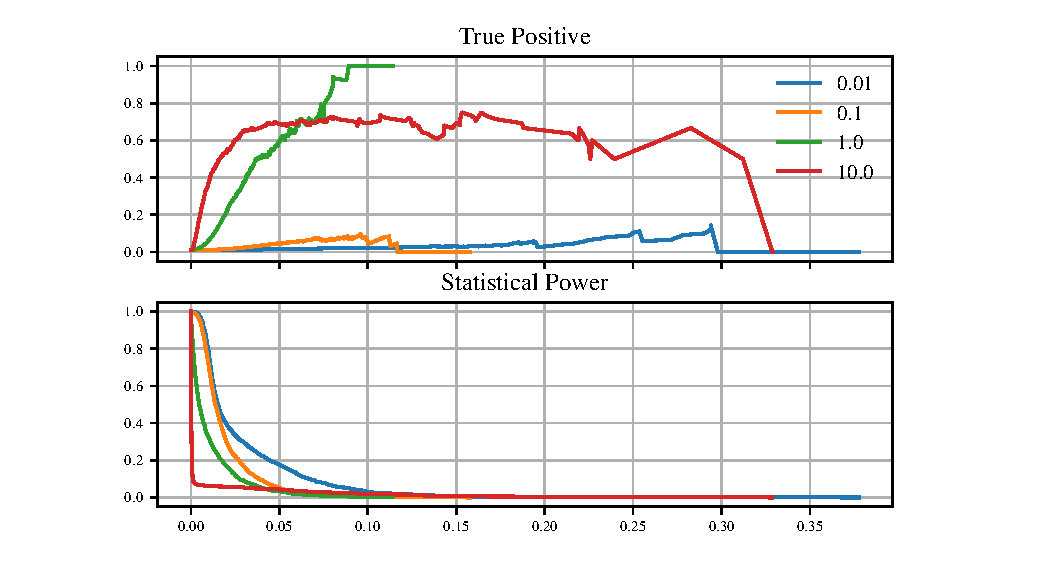
\includegraphics{Final_Plots/True_Power.pdf}
  		\caption{ 
		Statistical Power and False Positives as a function of $F_{st}$ threshold. 
		Statistical Power is the likelihood that a SNP will be predicted to have an effect on phenotype when there is an effect to be detected (?).
		False Positives give us the ratio of SNPs that effect phenotype to total SNPs greater than the $F_{st}$ threshold.
        		TODO: x-axis label ($F_{ST}$).
		}
  		\label{fig:Power_FP}
	\end{center}
\end{figure}

\begin{figure}
	\begin{center}
  		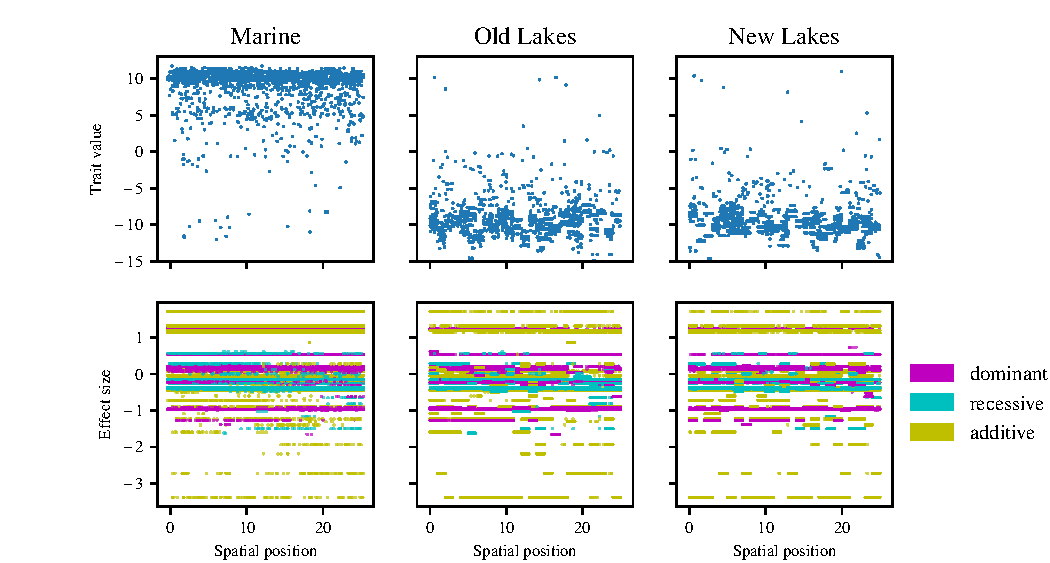
\includegraphics[width=1.0\linewidth]{Final_Plots/Haplo_small.pdf}
  		\caption{
			Phenotypes (\textbf{Top}) (effect size and mutation type) and haplotypes \textbf{(Botton)} as a function of spatial position of the individual 
			possessing the genome. The phenotype of each haplotype is, by definition, the sum of the 
			effect sizes of each mutation in the genome. 
		}
  		\label{fig:Haplo_Pheno}
	\end{center}
\end{figure}


\end{document}
